%%%% Better Poster latex template example v1.0 (2019/04/04)
%%%% GNU General Public License v3.0
%%%% Rafael Bailo
%%%% https://github.com/rafaelbailo/betterposter-latex-template
%%%% 
%%%% Original design from Mike Morrison
%%%% https://twitter.com/mikemorrison

\documentclass[a0paper,fleqn]{src/betterposter}

\begin{document}	
\betterposter{
%%%%%%%% MAIN COLUMN

\maincolumn{
%%%% Main space

\textbf{Main finding} goes here,
\\translated into \textbf{plain English}.
\\\textbf{Emphasize} the important words.
}{
%%%% Bottom space

%% QR code
\qrcode{img/metapackage/qrcode.png}{img/general/smartphoneBlack}{
\textbf{Want to see an example repository?} \\ \checkmark Check https:\slash \slash github.com/ansys/pyansys \\ \newline \textbf{Any doubts?} \\ \checkmark Don't be shy and start the conversation!
}
% Smartphone icon
% Author: Freepik
% Retrieved from: https://www.flaticon.com/free-icon/smartphone_65680

%% Compact QR code (comment the previous command and uncomment this one to switch)
%\compactqrcode{img/example/qrcode}{
%\textbf{Take a picture} to
%\\download the full paper
%}

}

}{
%%%%%%%% LEFT COLUMN

\title{Python \\metapackages}
\author{Roberto Pastor Muela}
\institution{Ansys}

\section{
\includegraphics[height=\fontcharht\font`\S]{img/general/slash.png} Introduction}
Organizations experience problems when distributing multiple packages. What if you could easily distribute
all your packages under one same package? Python \textit{metapackages} are here to solve your problems!

\section{
\includegraphics[height=\fontcharht\font`\S]{img/general/slash.png} The \textit{metapackage}\\concept}
Python \textit{metapackages} are empty Python libraries that only contain a version attribute.
However, they use their dependencies section to declare all the required libraries that need
to be installed. This trick can be used to install all the desired projects of a large community.

\section{
\includegraphics[height=\fontcharht\font`\S]{img/general/slash.png} Conclusion}
This is a great poster format!

%% This fills the space between the content and the logo
\vfill

%% Institution logo

\includegraphics[width=\textwidth]{img/general/pyansys_dark}\\

}{
%%%%%%%% RIGHT COLUMN

Here you can add \textbf{supplementary material}. For instance, a new diagram:
\begin{center}
% Commutative diagram with edges passing under/over
% Author: Stefan Kottwitz, http://texblog.net/
% Retrieved from: http://www.texample.net/tikz/examples/commutative-diagram/
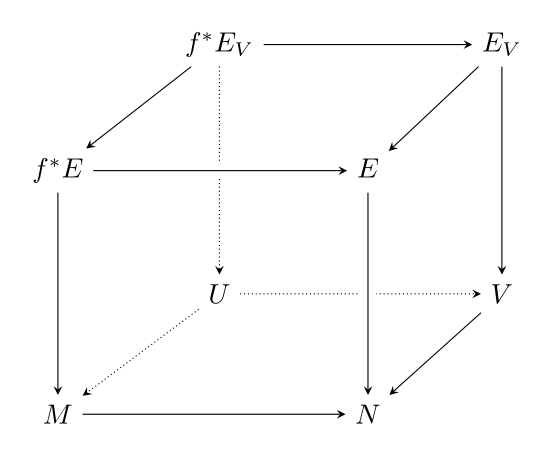
\includegraphics[width=\textwidth]{img/example/tikzexample2}
\end{center}

Some cute ducklings:
\begin{center}
% Picture of ducklings
% Author: Magda Ehlers, https://www.pexels.com/@magda-ehlers-pexels
% Retrieved from: https://www.pexels.com/photo/selective-focus-photo-of-flock-of-ducklings-perching-on-gray-concrete-pavement-1300355/
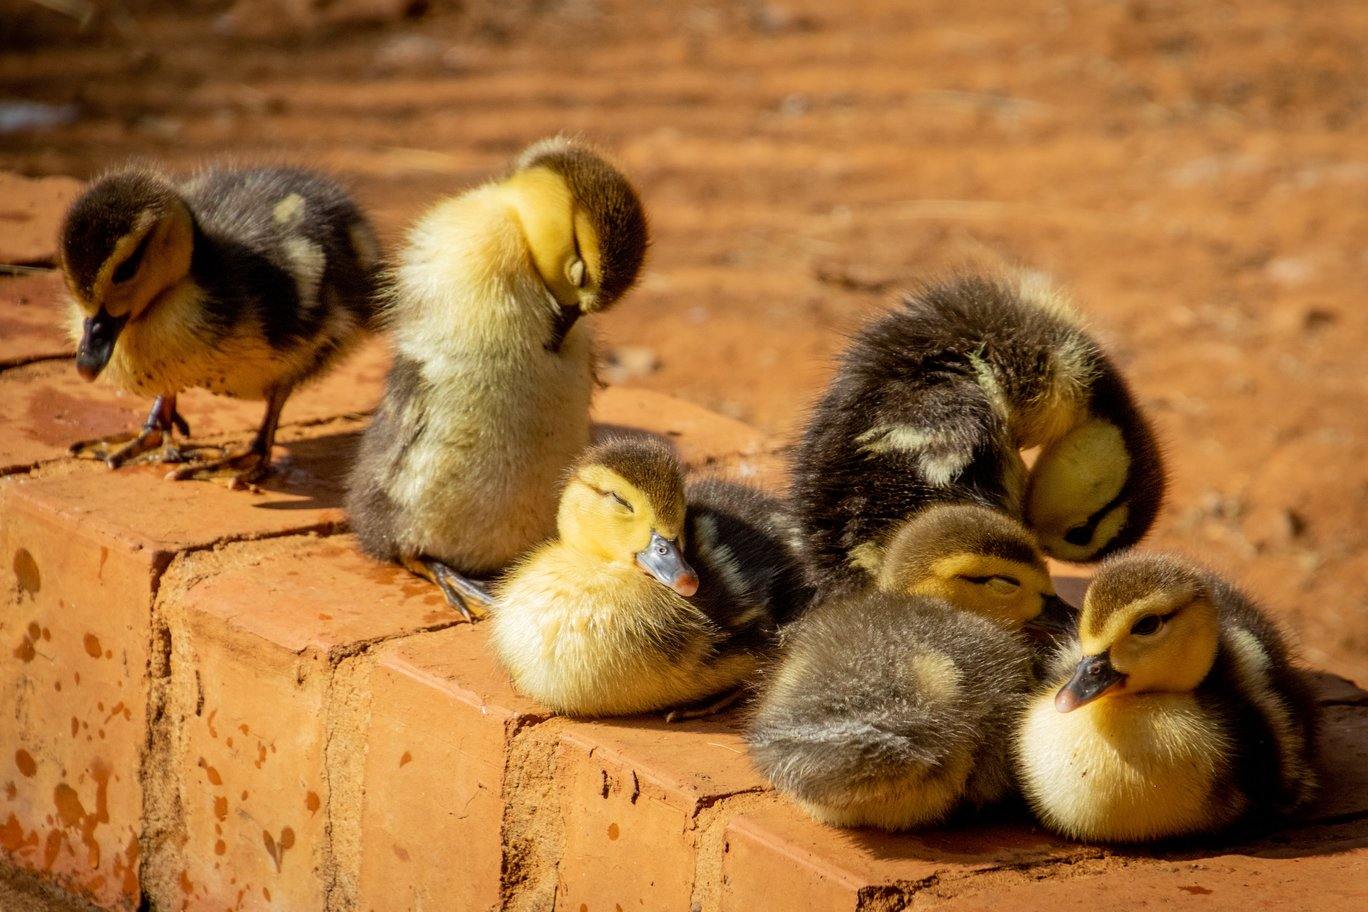
\includegraphics[width=\textwidth]{img/example/ducklings}
\end{center}

\section{
\includegraphics[height=\fontcharht\font`\S]{img/general/slash.png} What is PyAnsys?}
The PyAnsys project is a collection of Python packages that enable the use of Ansys products through Python.
Much effort is underway to continue expanding and developing repositories in the Ansys GitHub organization.
\\
\newline
\textbf{Any doubts?} \\Contact us at pyansys.core@ansys.com! We will be happy to help you out.
\\
\newline

\qrcode{img/general/pyansys_qrcode.png}{img/general/smartphoneBlack}{
\textbf{\huge{Check our docs for more\\information on PyAnsys!\\https:\slash \slash docs.pyansys.com }}
}
}
\end{document}
